\documentclass{scrartcl}
\usepackage{german}
\usepackage[utf8]{inputenc}
\usepackage[german]{babel}
\usepackage{amssymb}  % advanced mathematical symbold
\usepackage{graphicx} % using graphics
\usepackage{fancyhdr} % for the head of the page
\usepackage{lastpage} % makes page numbers work
\usepackage{listings} % for lstlistings
\usepackage[usenames, dvipsnames]{color}    % for color
\setlength{\parskip}{\medskipamount} % thats reasonable
\setlength{\parindent}{0pt}


\lstset{
    basicstyle=\ttfamily,
    mathescape
}

%%%%%%%%%%%%%%%%%%%%%%%%
% Kopf- und Fusszeilen %
%%%%%%%%%%%%%%%%%%%%%%%%
\pagestyle{fancy}
\lhead{
    \begin{tabular}{ll}
        Felix Karg & 4342014\\
    \end{tabular}
}
\chead{Graphentheorie}
\rhead{
    \begin{tabular}{rr}
        \today{} \\
        Seite \thepage{} von \pageref{LastPage}
    \end{tabular}
}
\lfoot{}
\cfoot{}
\rfoot{}

%%%%%%%%%%%%%%%%%%%%%%%%
% Anfang des Dokuments %
%%%%%%%%%%%%%%%%%%%%%%%%
\begin{document}

\section*{Antworten zu Übungsblatt Nr. 3}

\section*{Aufgabe 1}

\begin{itemize}
    \item[a)] topologische Sortierung von G: $\sigma(v_i) = i$
    \item[b)] $v_1$: 1, $v_2, v_3$: Faktor 2!x, $v_4, v_5:$ Faktor 2 * (2 + x) (mit 2 kombinationen von Folgezuständen, also 4, 6 für die beiden), $v_6, v_7, v_8$ pur: 3!, Summe: $2! * 2 * (2 + 3!) = 2 * 2 * (2 + 6) = 4 * 8 = 2^5 = 32$
    \item[c)] Algorithmus zur Berechnung der Anzahl der Topologischen Sortierungen
        \begin{lstlisting}
Beginnend bei einem Knoten mit $d^-(v) = 0$ und einer Zahl n = 0 führt man
folgende Schritte aus:
  solange valide Zustände vorhanden sind (die man noch nicht zuvor
  bereits belegt hatte), sucht man sich einen aus und versucht
  rekursiv alle Knoten Sinnvoll so zu belegen, wie sie in der
  Kombination noch nicht belegt waren. Sind alle belegt, Zählt man n
  += 1, und fängt wieder von vorne an, sind noch nicht alle Belegt
  aber es gibt keine Validen mehr (jede folgende Belegung wäre keine
  Topologische Sortierung) merkt man sich trotzdem welche man bereits
  belegt hat, aber fängt auch wieder von vorne an. Sollte es
  irgendwann nicht mehr möglich sein, neue sinnvolle Belegungen zu
  finden ist man Fertig und hat in $n$ die Anzahl der möglichen
  Topologischen Sortierungen.
        \end{lstlisting} \\
        Lösung: \\
        \begin{lstlisting}
count(G, i):
    if v(G) = $\emptyset$ then
        print $\sigma$
        return 1
    fi
    $L_0 = \{ v \in V(G) | g^-(v) = 0 \}$
    r = 0
    $\forall v \in L_0$ do
        $\sigma(v) = i$
        r := r + count(G - v, i+1)
    od
    return r

        \end{lstlisting}

% \begin{lstlisting}
% back :: [(n, v)]
% front :: queue(v_i)
% front.add( Menge an $v$ mit $d^-(v) = 0$);
% i32 i = 1;
% for v : front.pop() {
%     if (alle $\alpha(v)$ schon in back) {
%         front.add($\omega(v)$);
%         back.insert(i, v);
%         i += 1;
%     } else {
%         front.add({v});
%         // Funktioniert, fügt also für
%     }
% }
% return back;
% \end{lstlisting}

    \item[d)] (n-1)!, da der Knoten ohne eingehende Kanten die 1 zugewiesen
        bekommt und nun alle anderen keine Weiteren einschränkungen haben, also
        nur noch Permutationen sind.
    \item[e)] Maximale Anzahl Möglichkeiten topologischer sortierungen: \\
        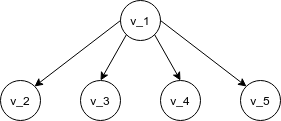
\includegraphics[width=7cm]{max_top.png} \\
        Minimale: \\
        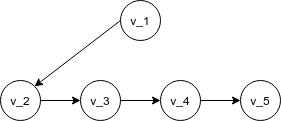
\includegraphics[width=7cm]{min_top.png}

\end{itemize}



\section*{Aufgabe 2}
Begriffe:
\begin{itemize}
    \item Einfach: ohne parallele Kanten oder Schleifen
    \item Kreis: Pfad mit selbem Start/Endknoten.
    \item {\color{blue} Eulersch}:  Es existiert ein Kreis der alle Kanten genau einmal besucht.
    \item {\color{ForestGreen} Hamiltonisch}: Es existiert ein Kreis der alle Knoten genau einmal besucht.
\end{itemize}

$G$ ist Zusammenhängender ungerichteter Graph mit $|V| \geq 2$.

\begin{itemize}
    \item[a)] $G$ enthält einen {\color{YellowOrange}Eulerschen}
        Kreis und einen {\color{YellowOrange}Hamiltonschen} Kreis: \\
        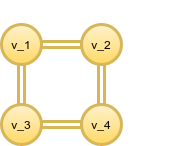
\includegraphics[width=4cm]{eul_ham.png}
    \item[b)] $G$ enthält weder einen
        {\color{blue}Eulerschen} Kreis noch einen
        {\color{ForestGreen}Hamiltonschen} Kreis: \\
        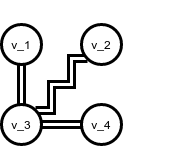
\includegraphics[width=4cm]{neul_nham.png}
    \item[c)] $G$ enthält einen
        {\color{blue}Eulerschen} Kreis, jedoch keinen
        {\color{ForestGreen}Hamiltonschen} Kreis: \\
        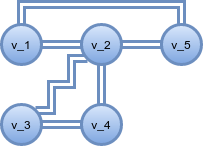
\includegraphics[width=4.5cm]{eul_nham.png}
    \item[d)] $G$ enthält
        keinen {\color{blue}Eulerschen} Kreis, jedoch einen
        {\color{ForestGreen}Hamiltonschen} Kreis: \\
        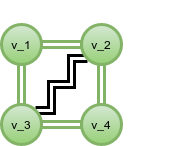
\includegraphics[width=4cm]{neul_ham.png}
\end{itemize}

% (Blau: Eulerscher Kreis, Grün: Hamilton'scher Kreis, Gelb: Beides, Schwarz: Weder noch)

\end{document}


